\newpage

\subsection*{Parity}

\begin{flushleft}
  Tras haber realizado mediciones de tiempo a las distintas funciones
  programadas en el archivo \textit{parity.c} los resultados fueron los
  siguientes:
\end{flushleft}

\begin{table}[!htbp]
\centering
\caption{Parity -O0}
\label{my-label}
\begin{tabular}{|l|l|l|l|l|l|l|l|l|l|l|l|}\hline
-O0      & 0    & 1    & 2    & 3    & 4    & 5    & 6    & 7    & 8    & 9    & Media \\\hline
Parity 1 & 6205 & 5642 & 5385 & 5219 & 5181 & 5112 & 5607 & 5518 & 6726 & 5110 & 5571  \\\hline
Parity 2 & 2845 & 2144 & 2174 & 2206 & 2738 & 2155 & 2223 & 2279 & 2773 & 2138 & 2368  \\\hline
Parity 3 & 2634 & 1898 & 1917 & 1955 & 2076 & 1886 & 1947 & 2487 & 2327 & 2028 & 2116  \\\hline
Parity 4 & 1140 & 738  & 668  & 693  & 1011 & 671  & 697  & 703  & 826  & 969  & 812   \\\hline
Parity 5 & 1021 & 908  & 825  & 852  & 967  & 820  & 1067 & 842  & 1009 & 1344 & 966   \\\hline
Parity 6 & 218  & 223  & 195  & 202  & 203  & 196  & 202  & 202  & 241  & 286  & 217   \\\hline
\end{tabular}
\end{table}

\begin{table}[!htbp]
\centering
\caption{Parity -O1}
\label{my-label}
\begin{tabular}{|l|l|l|l|l|l|l|l|l|l|l|l|}\hline
-O1      & 0    & 1    & 2    & 3    & 4    & 5    & 6    & 7    & 8    & 9    & Media \\\hline
Parity 1 & 3960 & 1365 & 1373 & 1525 & 1575 & 1348 & 1357 & 1345 & 1335 & 2574 & 1776  \\\hline
Parity 2 & 1885 & 669  & 637  & 1161 & 743  & 637  & 637  & 637  & 637  & 784  & 843   \\\hline
Parity 3 & 1914 & 657  & 684  & 824  & 756  & 696  & 657  & 657  & 658  & 834  & 834   \\\hline
Parity 4 & 2589 & 636  & 637  & 1017 & 728  & 637  & 637  & 636  & 637  & 783  & 894   \\\hline
Parity 5 & 381  & 349  & 350  & 467  & 399  & 349  & 349  & 350  & 349  & 430  & 377   \\\hline
Parity 6 & 56   & 55   & 55   & 62   & 63   & 55   & 54   & 55   & 55   & 68   & 58    \\\hline
\end{tabular}
\end{table}

\begin{table}[!htbp]
\centering
\caption{Parity -O2}
\label{my-label}
\begin{tabular}{|l|l|l|l|l|l|l|l|l|l|l|l|}\hline
-O2      & 0    & 1    & 2    & 3    & 4    & 5    & 6    & 7    & 8    & 9    & Media \\\hline
Parity 1 & 2527 & 1429 & 1417 & 1508 & 1495 & 1495 & 1750 & 1549 & 1549 & 1393 & 1611  \\\hline
Parity 2 & 545  & 530  & 463  & 483  & 483  & 495  & 568  & 531  & 619  & 531  & 525   \\\hline
Parity 3 & 371  & 371  & 371  & 408  & 397  & 472  & 559  & 437  & 374  & 370  & 413   \\\hline
Parity 4 & 679  & 710  & 681  & 761  & 725  & 725  & 764  & 751  & 682  & 668  & 715   \\\hline
Parity 5 & 281  & 279  & 282  & 300  & 300  & 295  & 305  & 311  & 287  & 273  & 291   \\\hline
Parity 6 & 57   & 57   & 57   & 61   & 61   & 61   & 62   & 62   & 55   & 55   & 59   \\\hline
\end{tabular}
\end{table}

\newpage
En la siguiente gráfica hemos representado los resultados obtenidos:

\begin{figure}[!htbp]
  \centering
  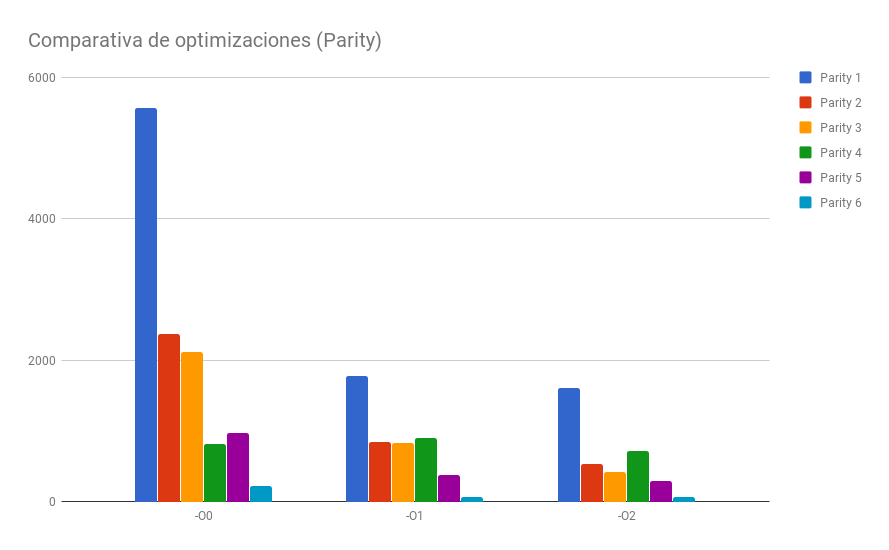
\includegraphics[width=1.1\textwidth]{parity.png}
\end{figure}
